\section{Azure Stream Analytics}
Wenn man an dem Punkt eines Prozesses angelangt ist, an welchem man eine große Menge von Daten gesammelt und zur Verfügung stehen hat, diese jedoch nur über einen (stark) begrenzten Zeitraum zurückgehalten werden können, bietet Azure Stream Analytics einen Dienst zur weiteren Verarbeitung, welcher nahtlos daran anknüpft. 


Vor allem im heutigen Industrie 4.0 Umfeld können solche Systeme einen großen Vorteil bieten. Es erlaubt beispielsweise Einblicke in die Sensordaten, um darin nach Mustern zu suchen und entsprechend darauf zu reagieren \cite{Klein.2017}. Eingehende Daten werden auf Anomalien oder je nach Aufgabe auf relevante Informationen analysiert. Die daraus resultierenden Ergebnisse werden daraufhin entsprechend Präsentiert. Benachrichtigungen werden hier in Echtzeit ausgelöst. Auch auf mobilen Geräten können diese geschickt werden. Ein typisches Echtzeitverarbeitungssystem, welches auf Stream Analytics und weiteren Azure-Diensten aufbaut, wird in Abbildung (…) illustriert.\\ \\
Dieser Service der Azure-Plattform kann Daten aus einem Datenstrom mit hoher Geschwindigkeit bearbeitet. Unterstützt wird dabei eine SQL-Ähnliche Abfragesprache Stream Analytics Query Language (SAQL), über welche man die dynamischen Datenströme analysiert. Diese ist das Herzstück von Azure Stream Analytics. Obwohl SAQL von der allgegenwärtigen SQL-Abfragesprache abgeleitet wurde, enthält es einzigartige Funktionen, die für die Stream-Verarbeitung notwendig sind \cite{Prosise.}. Eine dieser Funktionen ist die Möglichkeit, Ergebnisse mithilfe von Zeitfenstern zu erhalten (siehe Fensterfunktionen). 
\begin{figure*}[ht]
	\centering
	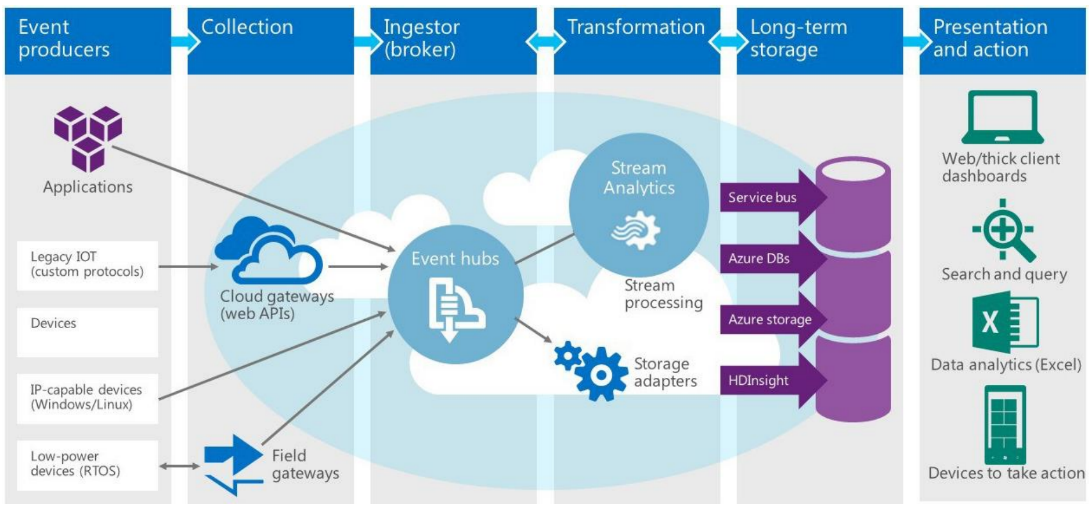
\includegraphics[width=0.8\textwidth,]{images/StreamAnalytics}
	\caption{Visualisierung der Probleme der einzelnen Bereiche\cite{Laukkanen.2017}.}
	\label{studie}
\end{figure*}
Die linke Spalte zeigt Sensoren einer IOT-Lösung, Geräte und andere Datenquellen. Diese senden kontinuierlich Daten über das Cloud Gateway an die Azure Hubs. Der Gateway-Dienst ist hierbei ein virtuelles Gerät und ermöglicht eine konsistente und leistungsfähige Verbindung. Die Hubs sind in der Lage Millionen von Ereignissen pro Sekunde zu verarbeiten. Von dort aus werden sie an die weiteren Anwendungen geliefert. Eine Anwendung, um eben diese Daten zu analysieren ist der Stream Analytics-Dienst. Dieser Dienst befindet sich in der Spalte der Transformation. Die Ausgabe kann hierbei auf eine Vielzahl von Endpunkten gerichtet werden. Azure bietet hier einige weitere Dienste, die hier angeknüpft werden können. Die rechte Spalte im Schaubild zeigt lediglich noch die Möglichkeiten, die Daten bzw. Ergebnisse darzustellen \cite{Prosise.} \\
Die Eingaben, die ein Stream Analytics-Job benötigt, können einfach im Azure-Portal konfiguriert werden. Eingaben können Azure-Event-Hubs, Azure-IoT-Hubs und Azure Blob-Speicher umfassen. Ein einzelner Stream Analytics-Job kann mehrere Eingaben enthalten. Es können Datenströme zusammengeführt werden, um die kombinierten Daten abzufragen. Dies ist kann mit einem JOIN in SQL verglichen werden. Auch die Ausgaben werden im Portal angegeben. Ausgaben können Kombinationen aus folgenden\\ \\ Komponenten sein:
\begin{itemize}
\item Azure-Blobspeicher 
\item Azure-Tabellenspeicher 
\item Azure-Ereignis-Hub 
\item Azure-Servicebus-Thema 
\item Azure Service Bus-Warteschlange 
\item Azure DocumentDB 
\item Microsoft Power BI 
\item Azure Data Lake Store \\ 
\end{itemize}
Diese breite Palette der unterstützten Ausgabetypen, die Azure hier anbietet, ermöglicht eine Menge an Szenarien. Beispielsweise könnten Aufzeichnungen des Stream Analytics-Job in den Azure Blob-Speicher, Azure-Tabellenspeicher, in eine SQL-Datenbank usw. dauerhaft gespeichert werden. Wenn Stream Analytics nun bei der Analyse des Datenstroms Auffälligkeiten oder Anomalien erkennt, können Push-Benachrichtigungen an diverse Geräte gesendet werden. Die Tatsache, dass ein einzelner Stream Analytics-Job mit mehreren Ein- und Ausgängen konfiguriert werden kann, ermöglicht umfangreiche Topologien mit durchgängigen Stream-Processing-Lösungen \cite{Prosise.}.